\documentclass{VUMIFPSkursinis}
\usepackage{algorithmicx}
\usepackage{algorithm}
\usepackage{algpseudocode}
\usepackage{amsfonts}
\usepackage{amsmath}
\usepackage{bm}
\usepackage{caption}
\usepackage{color}
\usepackage{float}
\usepackage{graphicx}
\usepackage{listings}
\usepackage{subfig}
\usepackage{wrapfig}
\usepackage{lithuanian}
\usepackage{longtable}

\usepackage{enumitem}
%PAKEISTA, tarpai tarp sąrašo elementų
\setitemize{noitemsep,topsep=0pt,parsep=0pt,partopsep=0pt}
\setenumerate{noitemsep,topsep=0pt,parsep=0pt,partopsep=0pt}

% Titulinio aprašas
\university{Vilniaus universitetas}
\faculty{Matematikos ir informatikos fakultetas}
\department{Programų sistemų katedra}
\papertype{Kursinis darbas}
\title{Labai panašių neuroninių klasių atskyrimas dirbtiniais neuroniniais tinklais}
\titleineng{(Separation of very similar neuronal classes by artificial neural networks)}
\status{3 kurso 5 grupės studentė}
\author{Miglė Vaitulevičiūtė}
\supervisor{dr. Vytautas Valaitis}
\date{Vilnius – \the\year}

% Nustatymai
% \setmainfont{Palemonas}   % Pakeisti teksto šriftą į Palemonas (turi būti įdiegtas sistemoje)
%\bibliography{bibliografija}
\documentclass{article}
\usepackage[backend=biber]{biblatex}
\addbibresource{bibliografija.bib}
\begin{document}
	
% PAKEISTA	
\maketitle
\cleardoublepage\pagenumbering{arabic}
\setcounter{page}{2}

%TURINYS
\tableofcontents

\sectionnonum{Įvadas}
Dirbtinių neuroninių tinklų idėja sugalvota buvo dar 1943 metais, bet dėl resursų trūkumo dirbtinių neuroninių tinklų efektyviai ir naudingai taikyti neišėjo. 
Tobulėjant technologijoms bei kompiuteriams galint vykdyti vis daugiau ir daugiau skaičiavimų dirbtiniai neuroniniai tinklai sparčiai įgijo populiarumą.

Vienas iš pagrindinių sprendžiamų uždavinių yra klasifikacija - tai yra paveiksliukų skirstymas į aprašytas klases. Tokį uždavinį atlieka dirbtinių neuroninių 
tinklų tipas - konvoliuciniai neuroniniai tinklai. Jie yra patys efektyviausi šio uždavinio sprendimui, kadangi jų įeities duomenys gali būti tik paveiksliukai.
Klasifikacijos uždavinys yra aktualus, kadangi jo panaudojimas yra labai skirtingas - nuo medicinos iki savi-vairuojančių mašinų.

Konvoliuciniai neuroniniai tinklai dar yra naudojami:
\begin{itemize}
\item Veido atpažinimui - identifikuoti arba verifikuoti asmenį. Pavyzdžiui, ,,DeepFace'' sistema sukurta ,,FaceBook'', kuri atpažįsta žmonių veidus nuotraukose 
arba ,,Face ID'' sistema sukurta ,,Apple'', kuri yra skirta identifikuoti asmenį, kuris bando atrakinti telefoną. 
\item Medicinoje - širdies, plaučių, prostatos vėžių ir akių ligų diagnozavimui.
\item Žmonių elgesio analizė realiu laiku - ,,DeepGlint'' nustato žmones nuotraukose ir nuspėja jų pozas.
\item Vertimas - ,,Google Translate'' gali versti tekstą iš paveiksliukų realiu laiku.
\end{itemize}

Daugiausia resursų išnaudojanti dirbinių neuroninių tinklų dalis yra mokymas. Šiai daliai reikia ne vien daug laiko - žmonių ir pačio mokymo, bet ir didelio 
paveiksliukų rinkinio, kuris privalo turėti aprašymus, kas pavaizduota juose. Tačiau realiame pasaulyje paveiksliukų kiekis ir žmogiškieji bei laiko resursai yra riboti, 
tad yra siekiama keičiant dirbtinio neuroninio tinklo architektūra, parametrus bei naudojamas funkcijas gauti kuo didesnį tikslumą bei mažiausią įmanomą nuostolį. 
Dirbtinio neuroninio tinklo teisingumą lemią ne vien kokybiški duomenys, didelį poveikį turi ir tinklo gylis - kiek daug sluoksnių turi dirbtinis neuroninis 
tinklas. 

Tad, šio darbo tikslas yra palyginti skirtinų gylių dirbtinius neuroninius tinklus pagal mokymosi tikslumą bei nuostolių dydį, kai mokymui yra naudojamas mažas 
paveikslėlių rinkinys ir keičiamos optimizavimo funkcijos.

Užduotys:
\begin{enumerate}
\item Pasirinkti naudojamą dirbtinio neuroninio tinklo architektūrą.
\item Sukurti programą, kuri reguliuotų ir modifikuotų jau egzistuojantį pasirinktos architektūros modelį.
\item Apmokyti reguliuotą ir modifikuotą modelį.
\item Palyginti SGD, Adam, Adagrad ir RMSprop optimizavimo funkcijas.
\end{enumerate}


\section{Dirbtinis neuroninis tinklas}
Pagal apibendrintą žmogaus smegenų veikimą buvo sugalvoti dirbtiniai neuroniniai tinklai \cite{Goodfellow-et-al-2016}. Bendrai žmogaus smegenys turi šimtus
milijardų neuronų, kurie yra sujungti sinapsėsmis. Per tuos neuronus sklinda elektroniniai impulsai perduodantys informaciją - taip žmonės gali 
atpažinti objektus, garsus ir t.t. Dirbtiniai neuroniniai tinklai veikia panašiai. Jie irgi turi daug besijungiančių neuronų, kurie gauna informaciją ir 
pagal tą informaciją gali nuspręsti koks objektas yra paveikslėlyje. Tačiau ties tuo ir baigiasi žmogaus smegenų ir dirbtinių neuroninių tinklų panašumas, 
kadangi dirbtiniai neuroniniai tinklai yra kompiuterinė simuliacija - matematinis algoritmas su aritmetiniais kintamaisiais. Ši simuliacija yra suvokiama 
tik žmogui, kuris suprogramavo dirbtinį neuroninį tinklą, pačiam tinklui simuliacija nieko nereiškia, nuovokos nesuteikia.

\subsection{Dirbtinio neuroninio tinklo sudėtis}
Dirbtinis neuroninis tinklas yra sluoksnių rinkinys (1 pav.) - neuronų grupė sudaro sluoksnį, kuris yra sujungtas tarpusavyje su kitais sluoksniais. Vienas iš
sluoksnių privalo būti įvesties sluoksnis, kuris atitinkamai pagal užduoti gali gauti įvairios formos informaciją - paveiksliukai, vaizdo
medžiaga, garsas ir t.t. Ši informacija yra reikalinga tam, kad tinklas galėtų ją išanalizuoti ir išmokti. Tuo tikslu, kad vėliau gavęs panašią
informaciją galėtų ją atpažinti - tam reikalingas išeities sluoksnis. Jis yra priešingame dirbtinio neuroninio tinklo gale negu įeities sluoksnis.
Tarp anksčiau apibūdintų sluoksnių yra įvairaus dydžio sluoksnių sistema, kuri atlieka pagrindinį darbą \cite{Woodford-2018}.

\begin{figure}[h]
\centering
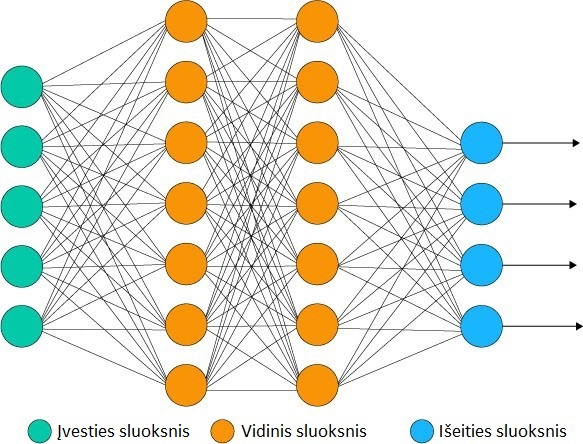
\includegraphics[width=0.5\textwidth]{img/NTSluoksniuSistema.jpeg}
\caption{Sluoksnių rinkinys}
\end{figure}

\subsection{Dirbtinio neuroninio tinklo veikimas}
Jungtys tarp neuronų yra pateiktos skaitine išraiška ir vadinamos svoriu. Kuo didesnis šis svoris tuo didesnę įtaką turi vienas neuronas kitam.
Vienam neuronui yra pateikiama visų prieš jį buvusių neuronų informacija ir jungčių svoriai. Kiekvieno neurono informacija yra sudauginama su
jo svoriu ir visi šie duomenys yra sudedami tarpusavyje. Taip iš vektoriaus gaunamas vienas rezultatas ir jei šis rezultatas tinka aktyvavimo
funkcijai, jis yra perduodamas tolimesniems neuronams. Tokio tipo veikimo dizainas yra vadinamas ,,feedforward'' tinklu.

Tačiau jungčių svoriai nėra pastovūs. Kai dirbtinis neuroninis tinklas mokosi, galutinis rezultatas yra lyginamas su tikėtinu teisingu rezultatu, jei šie
rezultatai skiriasi, svoriai yra keičiami atitinkamai, tai vadinama ,,backpropagation''. Tokiu būdu yra gerinamas rezultatas ir mažinamas skirtumas
tarp tikėtino ir gauto atsakymų.

\subsection{Aktyvavimo funkcijos}
Aktyvavimo funkcijų yra įvairių, kadangi sprendžiant tam tikrą problemą yra geriau naudoti vienas funkcijas, o kitas problemas - kitas funkcijas.
Pagrinde yra dviejų tipų aktyvavimo funkcijos - tiesinės ir netiesinės. Tiesinės nėra tokios populiarios, kadangi jos neleidžia įvesčiai
būti lanksčiai. Nors tiesinė funkcija labai dažnai naudojama išeities sluoksnyje.
Netiesinės funkcijos dažniausiai naudojamos vidiniuose sluoksniuose. Šiuo metu labiausiai naudojama yra ReLU, kadangi naudojant šią funkciją mokymo
rezultatai nuolatos gerėja, tačiau ReLU funkcijos spraustumas nesuteikia efektyvumo tinklui \cite{DBLP:journals/corr/XuWCL15}.

Aktyvavimo funkcijos yra skirstomos į:
\begin{itemize}
\item Tiesinė: 
\begin{itemize}
\item Žingsninė (binarinė) - išėjimas yra 0 arba 1.
\end{itemize}
\item Netiesinė: 
\begin{itemize}
\item Sigmoidinė - išėjimas intervale [0; 1].
\item Hiperbolinio tangento - išėjimas intervale [-1; 1].
\item Minkštojo maksimumo - sunormuoja išėjimo vektorių į 1.
\item ReLU - išėjimas intervale [0; begalybė].
\end{itemize}
\end{itemize}

Šio darbo eksperimento dalyje buvo naudotos ReLU ir sigmoidinė aktyvavimo funkcijos.

\subsection{Nuostolio funkcijos}
Kai dirbtinis neuroninis tinklas mokosi, jo gaunami rezultatai gali labai skirtis nuo tikėtinų rezultatų. Todėl nuostolio funkcija apskaičiuoja kaip stipriai
skiriasi gautas rezultatas nuo tikėtino. Kuo didesnis nuostolis tuo toliau nuo teisingo atsakymo yra dirbtinis neuroninis tinklas \cite{Cameron-loss-fun}.
Paprasčiausia ir dažniausiai naudojama nuostolio funkcija yra vidutinio kvadrato klaida. Ši funkcija apskaičiuoja kvadratinį skirtumą tarp tikėtino 
ir gauto rezultatų. Tačiau šios funkcijos vienas iš didesnių trūkumų - neproporcingas išskyrimas didelių rezultatų. Kadangi funkcija didėja kvadratiniai,
o ne tiesiniai, kai gaunamas rezultatas tolsta nuo tikėtino rezultato.

Priklausomai nuo to kokią problemą yra bandoma išspręsti yra naudojamos skirtingos funkcijos. Viena iš problemų yra klasifikacijos - dažniausiai išeities
rezultatas yra tikimybės vertė f(x). Bendrai, funkcijos reikšmės dydis parodo gauto rezultato tikslumą. Dauguma klasifikacijos nuostolių funkcijos stengiasi
maksimaliai padidinti tikslumą \cite{clas-loss-2017}. 


Kelios klasifikacijos nuostolio funkcijos:
\begin{itemize}
\item Binarinė kryžiaus entropija.
\item Neigiama registravimo tikimybė.
\item Maržos klasifikatorius.
\item Minkštų maržų klasifikatorius.
\end{itemize}

\subsection{Optimizavimo funkcijos}
Optimizavimo funkcijos naudojamos vidinių tinklo parametrų atnaujinimui, kad sumažinti gaunamų rezultatų netikslumą. 
Visos optimizavimo funkcijos gali būti suskirstytos į du tipus - nuolatinio mokymosi greičio ir prisitaikančio mokymosi. 
Lentelėje 1 išvardinti visos populiariausios optimizavimo funkcijos.

\begin{longtable}[h!]{ | p{2cm} | p{2.2cm} | p{2.5cm} | p{2.5cm} | p{4.5cm} | } 
\hline
Pavadinimas & Tipas & Privalumai & Trūkumai & Veikimas \\
\hline
SGD & Nuolatinio mokymosi greičio & Parametrų atnaujinimai turi aukštą dispersiją, kas leidžia lengviau rasti lokalų minimumą. & Didelis svyravimas trukdo konverguoti. & Parametrų atnaujinimas vykdomas kiekvienai mokymo iteracijai. \\
\hline
Adam & Prisitaikančio mokymosi & Greitai konverguoja ir modelio mokymosi greitis yra didelis bei efektyvus. & Praleidžia mažą lokalų minimumą. & Suskaičiuoja mokymosi greitį kiekvienam parametrui bei saugo eksponentiškai nykstantį prieš tai buvusį kvadratinio gradiento vidurkį ir eksponentiškai mažėjantį prieš tai buvusį gradiento vidurkį, panašų į momentą. \\
\hline
Adagrad & Prisitaikančio mokymosi & Nereikia rankiniu būdu derinti mokymosi greičio. & Mokymosi greitis visada yra mažėjantis ir nykstantis, kas lėtina konvergavimą. & Leidžia mokymosi greičiui priklausyti nuo parametrų. Dideli atnaujinimai nedažniems parametrams, maži atnaujinimai dažniems parametrams. \\
\hline
RMSprop & Prisitaikančio mokymosi & Greitai konverguoja. & Momentas nedidina funkcijos efektyvumo. & Dalija mokymosi greitį iš eksponentiškai nykstančio kvadratinio gradiento vidurkio. \\
\hline
\caption{Optimizavimo funkcijos}
\end{longtable}

Nuolatinio mokymosi greičio funkcijos turi hiperparametrą - mokymosi greitį. Jis privalo būti nustatytas, tačiau 
pasirinkti tinkamą mokymosi greitį gali būti sudėtinga - pasirinkus per mažą vidiniai parametrai gali labai lėtai 
konverguoti, o pasirinkus per didelį parametrams gali trukdyti konverguoti ir priversti nuostolio funkciją svyruoti
apie minimumą arba diverguoti. Šio tipo funkcijos turi panašų hiperparametrą - momentą - kuris didina mokymosi greitį, 
kai jis artėja prie minimumo. 

Vienos iš pagrindinių problemų nuolatinio mokymosi greičio funkcijų, kad jos privalo turėti nustatytus hiperparametrus 
iš anksto ir jie labai stipriai priklauso nuo modelio ir sprendžiamos problemos. Dar vienas trūkumas, kad toks pats 
mokymosi greitis yra pritaikomas visiems vidinių parametrų atnaujinimams.

Prisitaikančio mokymosi funkcijos turi atskirus kiekvieno parametro mokymosi greičio metodus, kurie teikia euristikos 
metodą, nereikalaujant brangaus darbo rankiniu būdu nustatant hiperparametrus mokymosi greičiui. Tačiau šios funkcijos 
generalizuoja blogiau negu nuolatinio mokymosi greičio funkcijos, nors ir mokymosi metu pasirodo geriau \cite{2017arXiv170508292W}.

% generalization -> http://www.ra.cs.uni-tuebingen.de/SNNS/UserManual/node16.html

\section{Konvoliucinis neuroninis tinklas}
Konvoliuciniai neuroniniai tinklai yra labai panašūs į paprastus dirbtinius neuroninius tinklus (daugiau informacijos skyriuje ,,Dirbtinis neuroninis
tinklas''). Tačiau pagrindinis skirtumas tarp šių tinklų yra, kad konvoliucinio įeities sluoksnis priima tik tai paveiksliukus, 
kurie jei padaryti su standartine skaitmenine kamera, turi tris komponentus - raudoną, žalią ir mėlyną. Šiuos komponentus galima 
įsivaizduoti kaip tris 2D matricas sudėtas viena ant kitos. Kiekvienos matricos i-osios eilutės ir j-ojo stulpelio elementas 
atitinka nuotraukos pikselį, kurio reikšmė yra intervale nuo 0 iki 255. Kadangi naudojamos informacijos tipas yra specifinis, 
tai labai sumažina tinklo parametrų kiekį ir tinklą padaro efektyvesnį.


Objektų atpažinimas paveiksliukuose yra sudėtingas dėl šių iššūkių:
\begin{itemize}
\item Segmentavimas - paveiksliukai gali atvaizduoti įvairias scenas, kuriose gali būti pavaizduota daug objektų, kurie vienas kita gali dalinai uždengti.
\item Šviesa - pikselių intensyvumas gali būti paveiktas šviesos šaltinio ar pačio objekto.
\item Deformacija - objektai gali būti deformuoti įvairiais būdais, pavyzdžiui, kiekvieno žmogaus ranka parašyti skaičiai skiriasi.
\item Galimybės - objektų klasės dažnai nustatomos pagal tai kaip patys objektai yra naudojami, pavyzdžiui, kėdės yra objektai sukurti sėdėti, tačiau jos gali turėti įvairų dizainą.
\item Žvilgsnio taškas - keičiant vietą iš kurios yra žiūrima gali keistis objekto forma, informacija šokinėja per įeities sluoksnio dimensiją (t.y. pikselius). 
\end{itemize}

\subsection{Konvoliucija}
Konvoliucija yra matematinė operacija, kuri apibūdina taisyklę, kuri parodo kaip reikia sujungti du informacijos rinkinius \cite{Convolution-book}. 
Paveiksliukų analizėje, statinė ir pagrindinė funkcija yra įeities paveiksliukas, kuris yra analizuojamas, o antroji, judanti funkcija, žinoma 
kaip filtras, nes ji išskiria paveiksliuko ypatybę. Abi funkcijos yra susietos daugyba (2 pav.). 

\begin{figure}[h]
\centering
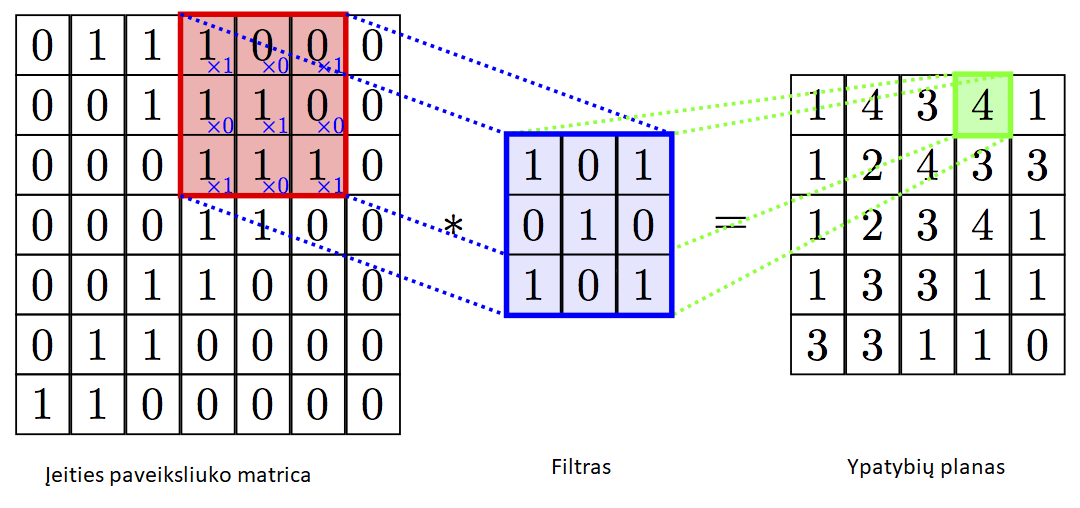
\includegraphics[width=0.5\textwidth]{img/Konvoliucija.png}
\caption{Konvoliucijos veikimas}
\end{figure}

Tačiau konvoliuciniai tinklai turi daug filtrų, kurie pereina per vieną paveiksliuką, kiekvienas išskirdamas skirtingą paveiksliuko ypatybę.
Pirmuose sluoksniuose šiuos filtrus galima įsivaizduoti kaip horizontalių, vertikalių ar įstrižų linijų filtrus, kurie sukuria paveikslėlio 
kraštų planą. Tinklas paima visus filtrus, gabaliukus paveiksliukų ypatybių vietų, ir juos sudeda į planą, kuris parodo ypatybės vietą. 
Mokydamasis skirtingų proporcijų ypatybių, tinklas leidžia lengvai kurti greitą ypatybių atpažinimą.

\subsection{Konvoliucinio neuroninio tinklo sluoksniai}
Konvoliuciniai neuroniniai tinklai tai yra sluoksnių rinkinys, kuris turi įeities, vidinius ir išeities sluoksnius. Tačiau priklausomai 
kokio tipo konvoliucinis neuroninis tinklas vidiniai sluoksniai gali skirtis. Konvoliuciniai neuroniniai tinklai turi tris pagrindinius 
sluoksnių tipus, kurie sudaro vidinį sluoksnį. Šie tipai yra konvoliucinis, sujungimo ir pilno sujungimo sluoksniai.

\subsubsection{Konvoliucinis sluoksnis}
Šis sluoksnis yra pagrindinis konvoliucinio neuroninio tinklo sluoksnis, kuris atlieka daugiausia skaičiavimų, nustato visas paveiksliuko ypatybes.
Kadangi, įeities informacija (paveiksliukas) yra didelės dimensijos neefektyvu visų neuronų sujungti vienus su kitais. Todėl neuronai yra sujungiami
su lokaliu informacijos kiekiu, kuris yra lygus filtro dydžiui ir vadinamas erdviniu mastu \cite{layers-CS231n}.

Neuronų kiekis po konvoliucijos (ypatybių plano dydis) yra nustatomas trimis parametrais:
\begin{itemize}
\item Gylis - atitinka filtrų skaičių.
\item Žingsnis - pikselių kiekis, kuris parodo per kiek reikia slinkti filtro matrica per įeities informacijos matricą.
\item Nulių pamušalas - įeities informacijos matricos kraštus užpildyti nuliais.
\end{itemize}


\subsubsection{Sujungimo sluoksnis}
Periodiškai sujungimo sluoksnis yra įterpiamas tarp konvoliucinių. Pagrindinis sluoksnio tikslas yra laipsniškai mažinti erdvinį filtruojamo paveiksliuko mąstą.
Šis veiksmas yra atliekamas tam, kad sumažinti parametrų ir skaičiavimų kiekį bei kontroliuoti perjungimą. Sujungimo sluoksnis veikia nepriklausomai nuo kiekvieno
gabalėlio gylio ir keičia jo dydį erdviškai, naudodamas MAX operaciją. Dažniausiai šis sluoksnis yra naudojamas su 2x2 dydžio filtru - kas antras po konvoliucijos 
gauto gabaliuko kiekvienas gylio sluoksnis yra mažinamas per pusę ties ilgiu ir pločiu, taip yra atsikratoma 75 procentų aktyvacijų. Po šios operacijos gabaliuko 
gylis nepasikeičia.

Dažniausiai yra naudojamos dvi šio sluoksnio variacijos. Pirmasis yra vadinamas persidengiantis sujungimas, kur filtro dydis yra lygus 3 ir žingsnis yra lygus 2. 
O kitas dažniau naudojamas turi filtro dydį lygų 2 ir žingsnį taip pat 2. Sujungimo sluoksniai su labai dideliais parametrais yra labai destruktyvūs.

\subsubsection{Pilno sujungimo sluoksnis}
Konvoliucinio ir sujungimo sluoksnių išeitys yra aukšto lygio ypatybės, kurios yra gautos iš įeities paveiksliuko. Pilno sujungimo sluoksnis yra sujungtas su visais 
neuronais iš sluoksnio buvusio prieš jį. Šio sluoksnio tikslas yra panaudojant tas ypatybes, kurios yra gautos iš prieš tai buvusių sluoksnių, nustatyti kokioms 
klasėms priklauso įeities paveiksliukas pagal mokymo informacijos rinkinį, kai neuroninio tinklo problema yra klasifikacija \cite{layers-fullyconnected}. Jei šiam sluoksniui yra naudojama 
minkštojo maksimumo funkcija tuomet sudėtis visų gautų galimybių turi būti lygi 1. Minkštojo maksimumo funkcija priima vektorių įvertinimų ir jį suspaudžia į 
vektorių, kuriame yra klasių tikimybių įvertinimai intervale nuo 0 iki 1, kur tikimybė arčiausiai vieneto reiškia, kad labiausiai užtikrintas dėl tos klasės.

\subsection{Architektūros}
Konvoliuciniai neuroniniai tinklai turi keletą skirtingų architektūrų, kurios yra naudojamos atitinkamai pagal sprendžiamą problemą. 1 lentelėje pateikta informaciją 
apie įvairias architektūras.


\begin{longtable}[h]{ | p{4cm} | p{1cm} | p{3cm} | p{5cm} | p{1.5cm} | } 
\hline
Pavadinimas & Metai & Parametrų kiekis & Veikimas & ILSVRC vieta \\
\hline
LeNet & 1998 & 60 000 & Geriausiai atpažįsta ranka parašytus skaičius. Susideda iš sluoksnių - kelių pasikartojančių konvoliucijos ir sujungimo bei pasibaigia dviem pilno sujungimo sluoksniais. & - \\
\hline
AlexNet & 2012 & 60 000 000 & Veikimu panašus į LeNet, tačiau turi daug daugiau parametrų ir filtrų bei sudėtus konvoliucinius sluoksnius.  & pirma \\
\hline
GoogLeNet/Inception & 2014 & 4 000 000 & Vidiniai sluoksniai sudėti paraleliai, naudojami Inception moduliai. Vienas modulis savyje turi 1x1, 3x3 ir 5x5 dydžių konvoliucijos filtrų bei vidurkio sudėjimo sluoksnius. & pirma \\
\hline
VGGNet & 2014 & 138 000 000 & Panašus veikimas į AlexNet, tačiau daug gilesnis. Naudojamų filtrų dydis yra 3x3 ir jie yra sudėti vienas po kito. & antra \\
\hline
ResNet & 2015 & 25 000 000 & Turi labai daug sluoksnių, sudėtų vienas po kito, kurie turi liekamąjį bloką, kuris įeities informaciją perduoda tolimesniam sluoksniui ją pridėdamas ir taip sumažina konvoliucijos ir aktyvavimo funkcijų kiekį.  & pirma \\
\hline
\caption{Konvoliucinių neuroninių tinklų architektūros}
\end{longtable}

\subsection{Modelio reguliavimas}
Pilnas konvoliucinio neuroninio tinklo apmokymas gali užtrukti labai ilgą laiką ir išnaudoti daug resursų. Todėl yra kai kurios įstaigos arba žmonės, kurie apmoko savo 
tinklą ir jo svorius bei reikšmes, vadinamą modeliu, pateikia visuomenei, tačiau šis modelis yra nepritaikytas individualiai žmogaus užduočiai. Modelį reikia 
reguliuoti - iš naujo apmokyti paskutinius sluoksnius su individualios užduoties parametrais.

Daugelis konvoliucinių neuroninių tinklų apmokytų su natūraliais paveiksliukais turi fenomeną. Pirmuosiuose sluoksniuose jie išmoksta ypatybių panašių į Gaboro filtrą 
(tiesinis filtras naudojamas tekstūroms analizuoti) ir spalvų dėmes. Šios pirmojo sluoksnio ypatybės nepriklauso nuo duomenų rinkinio, bet yra bendros ir tinkamos 
daugeliui duomenų rinkinių ir užduočių \cite{DBLP:journals/corr/YosinskiCBL14}. Dėl šio fenomeno galima naudoti modelius neapmokytus su specifiniu duomenų rinkiniu, 
bet jį minimaliai modifikuotą, kitoms užduotims spręsti, kas leidžia sutaupyti resursų bei turėti mažesnį duomenų rinkinį.

\section{Technologijos}
Naudojamų technologijų išsirinkimas yra pradinis žingsnis siekiant įvykdyti išsikeltas užduotis. Šiame skyriuje pateiktos populiariausios šių laikų technologijos 
bei trumpai papasakota apie jas.

\subsection{ImageNet}
ImageNet yra projektas sugalvotas profesorės Li Fei-Fei 2009 metais. Projekto tikslas buvo sukurti didelę sukategorizuotų paveiksliukų ir jų etikečių duomenų bazę, 
kuri butų skirta vizualinio objekto atpažinimo programinės įrangos tyrimams. Ši duomenų bazė yra suorganizuota pagal WorldNet hierarchija - anglų kalbos žodžiai 
yra grupuojami į sinonimų rinkinius, kurie turi apibūdinimus ir naudojimo pavyzdžius bei saugo ryšių kiekį tarp sinonimų arba jų narių. ImageNet turi daugiau nei 
100 000 sinonimų rinkinių, kur didžioji dalis yra daiktavardžiai (80 000+). 

Taip pat šis projektas kiekvienais metais daro konkursą vadinamą ,,ImageNet Large Scale Visual Recognition Challenge'' (trumpinys ILSVRC). Konkurso užduotis yra 
išmokinti modelį, kuris galėtų įeities paveiksliuką teisingai klasifikuoti į 1000 skirtingų objektų klasių, kurios atitinka realius daiktus, gyvūnus ir t.t. Modeliai 
yra apmokomi su apie 1.2 milijonų paveiksliukų ir dar 50 000 paveiksliukų yra naudojami validacijai mokymo metu bei 100 000 paveiksliukų yra panaudojami galutiniam 
modelio testavimui. Šis konkursas yra paveiksliukų klasifikacijos algoritmų etalonas.

\subsection{Keras}
Keras yra aukšto lygio programų sąsaja skirta neuroniniams tinklams. Sąsaja parašyta su ,,Python'' programavimo kalba ir vidinėje pusėje galinti veikti su ,,TensorFlow'' 
ir kitomis bibliotekomis. Keras buvo sukurtas tikintis suteikti greitą eksperimentavimą, kad sugalvojus idėją pasiekti rezultato būtų galima su kiek įmanoma mažiau uždelsimo.

Ši sąsaja savyje turi visus pagrindinius neuroninio tinklo kūrimo blokus, pavyzdžiui, sluoksniai, aktyvavimo ir optimizavimo funkcijos. Taip pat Keras suteikia modelius, 
kurie yra apmokyti naudojant ImageNet duomenų bazę. Šiuos modelius galima reguliuoti, pridėti papildomų sluoksnių, pasirinkti esamus sluoksnius bei juos iš naujo apmokyti.

\subsection{TensorFlow}
TensorFlow yra atviros programinės įrangos biblioteka skirta aukšto našumo skaitiniams skaičiavimams. Jo lanksti architektūra leidžia lengvai diegti skaičiavimus įvairiose 
platformose - procesoriuose, grafikos procesoriuose. Sukurtas ,,Google'' dirbtinio intelekto skyriaus, tad yra labai palaikomas automatinis ir gilusis mokymasis, tačiau 
dėl bibliotekos ir skaičiavimų lankstumo yra naudojamas įvairiose mokslinėse srityse.

\section{Eksperimentas}
Šio eksperimento tikslas yra išanalizuoti mokymosi tikslumą su skirtingų gylių neuroninais tinklais, kai mokymui yra naudojamas mažas paveikslėlių rinkinys. Taigi, pirmas 
šio eksperimento žingsnis - išsirinkti konvoliucinį neuroninį tinklą. Poskyriuje ,,Architektūros'' yra trumpai apibūdinti pagrindiniai konvolicinių neuroninių tinklų tipai. 
Iš jų buvo išsirinktas VGG, kadangi jo veikimas ir sluoksnių išsidėstymas yra tinkamiausi išsikeltam tikslui įgyvendinti. Buvo nuspręsta daryti paprastą, binarinę paveikslėlių 
klasifikaciją - nustatymas ar katė, ar šuo pavaizduotas paveikslėlyje.

\subsection{Duomenų rinkinys}
Šiais laikais konvoliuciniai neuroniniai tinklai pranoksta prieš tai buvusias naujausias technologijas naudotas paveiksliukų klasifikacijai. Viena iš pagrindinių priežasčių 
yra dideli ir gerai aprašyti duomenų rinkiniai, kaip kad ImageNet duomenų bazė. Geriausiai tinklas pasirodo, kai yra apmokomas su bendromis ypatybėmis ir dar efektyviau 
pasirodo kai yra sureguliuoti su specifiniu duomenų rinkiniu \cite{DBLP:conf/eccv/ChuMBHD16}. Optimalus duomenų kiekis, kad gerai sureguliuoti 
modelį yra apie 10 000 paveiksliukų. 

Tačiau realybėje visų klasių objektų paveiksliukų nėra be galo daug, kadangi reikia skirti labai daug laiko ir žmogiškųjų resursų paveiksliukų žymėjimui bei turėti tiek 
daug paveiksliukų. Todėl tenka tinklus apmokyti su limituotais duomenų rinkiniais. Pagal šią realaus pasaulio problemą buvo įvykdyta viena iš eksperimento tikslo sąlygų - 
mažas duomenų rinkinys. Buvo surastas ir naudotas duomenų rinkinys, kuris turi 10 000 paveikslėlių - 8 000 mokymosi tikslui ir 2 000 validacijos.

\subsection{Programos veikimas}
Skyriuje ,,Technologijos'' yra išvardintos visos technologijos, kurios buvo naudotos šio eksperimento programai parašyti.

Pirmiausiai reikia paruošti kompiuterį darbui - įrašyti ,,Python'' programavimo įrankius, paruošti ,,Anaconda'' komandinę eilutę, ,,NVIDIA CUDA'' įrankius, Keras ir 
TensorFlow. Tačiau kompiuteris privalo turėti tinkamą procesorių ar grafinį procesoriaus bloką - kompiuteris, kurį naudojau turėjo Nvidia 1080 Ti. Programa, kuri 
reguliuoja modelį ir modifikuoja, nelabai skiriasi, tad dėstysiu modelio reguliavimo eigą, kuri bus vėliau pritaikyta ir modifikavimo daliai. 

Modelio reguliavimui pirmiausia reikia turėti modelį, kurį galima reguliuoti. Keras pateikia modelius, apmokytus su ImageNet, ir jų svorius, tad reikia tik importuoti 
tinkamą modelį - šiuo atveju VGG16. Importavimo metu reikia nustatyti, kad pilnai sujungtas sluoksnis nebūtų pridėtas, kadangi tada galime parinkti kokių dimensijų 
paveiksliukus naudosime ir kiek spalvų sluoksnių jie turės (standartiniai paveiksliukai turi 3). Tuomet reikia nustatyti kokius importuoto modelio sluoksnius norime 
mokinti ir kuriuos - ne. Iš visų esamų sluoksnių mokinimui nustačiau tik paskutinius 4, kadangi jie yra atsakingi už specifinių ypatybių išmokimą. Po šių egzistuojančio 
modelio paruošimų reikia sukurti naują Kero modelį, prie kurio reikia pridėti paruoštą egzistuojantį modelį bei pridėti kelis kitus sluoksnius tam tikru išsidėstymu - 
plokštinimo, tankumo, išmetimo ir tankumo. Pirmasis išmetimo sluoksnis turi aktyvacijos funkciją ReLU, o paskutinis - sigmoidinę. Po visų sluoksnių pridėjimo modelis iš 
viso turėjo 40 406 849 parametrų, iš kurių mokinami buvo 32 771 585, o tik 7 635 264 buvo nekeičiami. 

Naudotų sluoksnių paaiškinimai:
\begin{itemize}
\item Plokštinimo sluoksnis - skirtas tam, kad įeinančius duomenis suploti į atitinkamą sluoksnių skaičių, jeigu sluoksnio parametras nenustatytas suplojama į vieną sluoksnį.
\item Tankumo sluoksnis - atlieka tokią pačią funkciją kaip kad pilno sujungimo sluoksnis (daugiau informacijos poskyriuje ,,Pilno sujungimo sluoksnis'').
\item Išmetimo sluoksnis - sluoksnyje atsitiktinai yra išjungiami tam tikri neuronai su Bernulio pasiskirstymo tikimybe. Dažniausiai nustatytas 50 procentų.
\end{itemize}

Po modelio paruošimo, reikia nustatyti kokio dydžio paveikslėlių paketais bus mokomas ir validuojamas modelis. Kadangi partijų dydį reikia nustatyti pagal kompiuterio atmintį, 
po parametras bandymų buvo nustatyta, kad geriausi dydžiai yra mokymosi partijai 100 paveikslėlių, o validacijos - 25.
Tuomet nustatomas paveikslėlių aplankalo kelias, jų ir partijos dydis bei nustatomas klasės režimas į binarinį, nes duomenų rinkinys susideda iš dviejų klasių - kačių ir šunų.

Paruošę modelį bei paveikslėlių rinkinį, galima pradėti mokinti ir validuoti modelį. Taigi, nustatomas modelio kompiliavimo metodas, kur turi būti - nuostolio ir 
optimizavimo funkcijos. Daugiau apie nuostolio ir optimizavimo funkcijas galima skaityti skyriuose ,,Nuostolio funkcijos'' ir ,,Optimizavimo funkcijos''. Tačiau nuotolio 
funkcija šiame modelyje yra binarinė kryžiaus entropija bei ji yra nekeičiama viso eksperimento metu. Šio eksperimento metu bus naudojamos keturios optimizavimo funkcijos - SGD, 
Adam, Adagrad ir RMSprop. Po modelio sukompiliavimo yra aprašomas mokymo metodas, kuriam turi būti pateikta - paruošti paveiksliukai, žingsnis per epochą, epochų kiekis, 
paruošti validacijos paveiksliukai ir jų žingsnis. Taigi, šiame eksperimente epocha yra nustatyta 80, kadangi tokia išeina pagal visų turimų paveiksliukų skaičių ir paketo dydį.

Modelio modifikavimo veikimas yra toks pats išskyrus, kad pridedami ne 4 sluoksniai, o 14 sluoksnių, kurie visi yra tankumo sluoksniai su aktyvacijos funkcija ReLu. Jie yra 
pridedami tarp plokštinimo ir kito tankumo sluoksnio. Po visų sluoksnių pridėjimo iš viso buvo 51 952 449 parametrų, iš kurių buvo 44 317 185 mokinami, o tiek pat buvo nemokinami 
kaip ir reguliuojant modelį. Taigi, modifikavimo metu prisidėjo papildomi 11 545 600 parametrų.

\subsection{Modelių mokymas}
Parašius programas, kurios reguliuoja bei modifikuoja modelį, buvo pradėta jį mokyti ir validuoti su skirtingomis optimizavimo funkcijomis.
Mokymosi greitis buvo išrinktas 1e-4, kas yra 0.0001.
\subsubsection{Modelio reguliavimas}
Pasirinkta buvo pradėti eksperimentą nuo modelio modifikavimo, kadangi tokiu būdu galima pamatyti kaip modelio paskutiniai keli sluoksniai yra apmokomi ir kaip tikslumas ir nuostolis 
keičiasi mokymo metu, kai yra naudojamas negilus modelis.

Taigi, pirmiausiai buvo pasirinkta SGD optimizavimo funkcija. Apmokius modelį buvo gauti grafikai - 3 ir 4 paveiksliukai.

\begin{figure}[!htbp]
  \centering
  \begin{minipage}[b]{0.49\textwidth}
    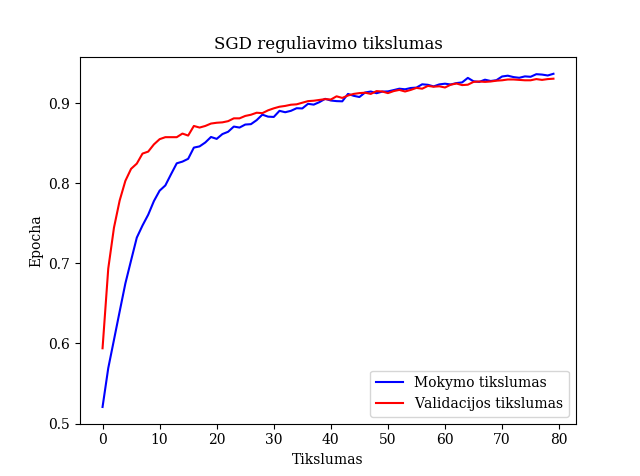
\includegraphics[width=\textwidth]{img/FT/SGD_acc.png}
    \caption{Modelio mokymosi ir validacijos tikslumas naudojant SGD}
  \end{minipage}
  \begin{minipage}[b]{0.49\textwidth}
    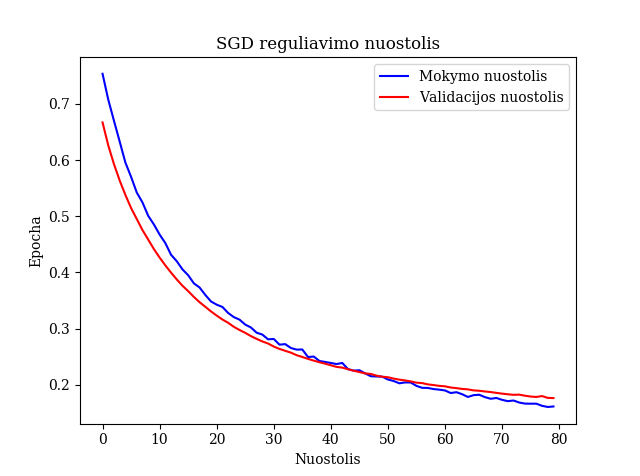
\includegraphics[width=\textwidth]{img/FT/SGD_loss.png}
    \caption{Modelio mokymosi ir validacijos nuostolis naudojant SGD}
  \end{minipage}
\end{figure}

Grafikas (3 pav.) parodo, kad tikslumas kyla kuo daugiau modelis išmoksta ir validacijos funkcija pirmiausiai pranoksta mokymosi, bet vėliau susilygina. Aukščiausias tikslumo rezultatas yra apie 94 procentus.
Bei grafikas (4 pav.) rodo nuostolį per epochas. Tad, jis parodo, kad mokymosi ir validacijos nuotoliai ties 47 epocha susikerta ir validacijos nuostoliai tampa didesni už mokymosi.

Paskui keičiama optimizavimo funkcija į Adam - mokymosi rezultatai matomi grafikuose - 5 ir 6 paveiksliukuose.

\begin{figure}[!htbp]
  \centering
  \begin{minipage}[b]{0.49\textwidth}
    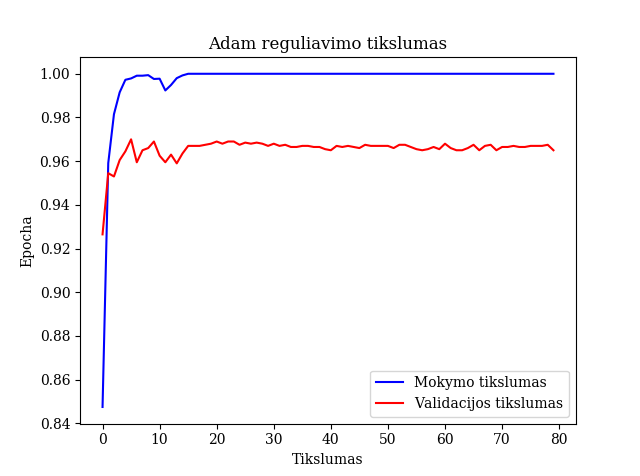
\includegraphics[width=\textwidth]{img/FT/Adam_acc.png}
    \caption{Modelio mokymosi ir validacijos tikslumas naudojant Adam}
  \end{minipage}
  \begin{minipage}[b]{0.49\textwidth}
    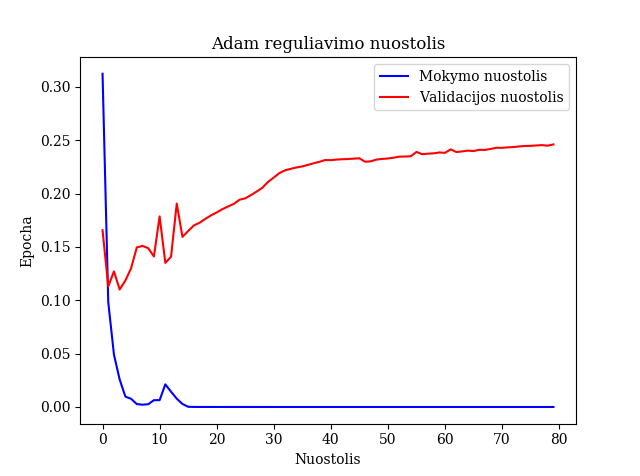
\includegraphics[width=\textwidth]{img/FT/Adam_loss.png}
    \caption{Modelio mokymosi ir validacijos nuostolis naudojant Adam}
  \end{minipage}
\end{figure}

Tikslumo grafikas (5 pav.) parodo, kad mokymosi tikslumas per kelias pirmas epochas pasiekia beveik 100 procentinį tikslumą, tačiau validacijos lieka apie 96 procentus ir daugiau nebekyla.
O nuostolio grafikas (6 pav.) parodo, kad mokymosi nuostolis staigiai nukrenta iki beveik 0 procentų nuostolių. Tačiau validacijos nuostoliai per kelias epochas nukrenta, o po to staigiai pradeda augti ir išsilygina ties 24 procentais.

Trečiasis testuojama optimizavimo funkcija yra Adagrad. Jos grafikai yra 7 ir 8 paveiksliukai.

\begin{figure}[!htbp]
  \centering
  \begin{minipage}[b]{0.49\textwidth}
    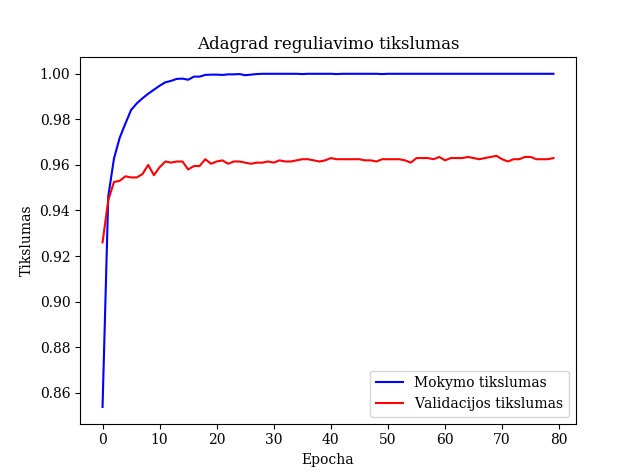
\includegraphics[width=\textwidth]{img/FT/Adagrad_loss.png}
    \caption{Modelio mokymosi ir validacijos tikslumas naudojant Adagrad}
  \end{minipage}
  \begin{minipage}[b]{0.49\textwidth}
    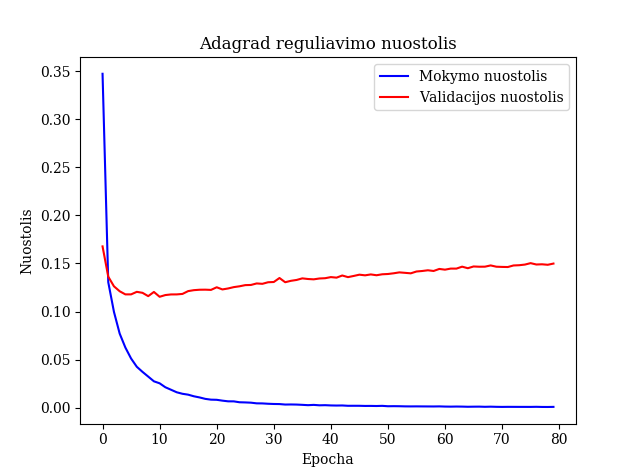
\includegraphics[width=\textwidth]{img/FT/Adagrad_acc.png}
    \caption{Modelio mokymosi ir validacijos nuostolis naudojant Adagrad}
  \end{minipage}
\end{figure}

Taigi, tikslumo grafikas (7 pav.) parodo, kad mokymosi tikslumas per pirmas 20 epochų pakyla beveik iki 100 procentų, o validacijos tikslumas pakyla iki 96 procentų ir ties tiek pasilieka.
O nuostolio grafikas (8 pav.) parodo, kad taip pat kaip ir mokymosi tikslumas taip ir nuostolis per pirmas 20 epochų nukrenta iki beveik 0 procentų ir ties ten lieka. Kai validacijos nuostolis 
nukrenta iki tolygiai auga iki 11 procentų, o po to tolygiai kyla iki 15 procentų.

Paskutinis bandymo optimizavimo funkcija yra RMSprop. Ji yra parodyta 9 ir 10 paveiksliukuose.

\begin{figure}[!htbp]
  \centering
  \begin{minipage}[b]{0.49\textwidth}
    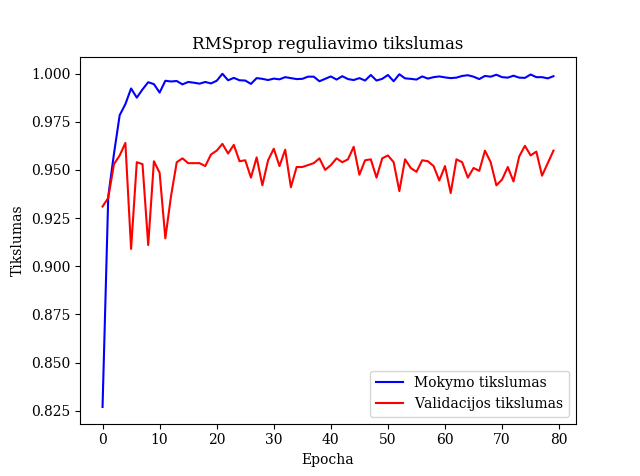
\includegraphics[width=\textwidth]{img/FT/RMSprop_acc.png}
    \caption{Modelio mokymosi ir validacijos tikslumas naudojant RMSprop}
  \end{minipage}
  \begin{minipage}[b]{0.49\textwidth}
    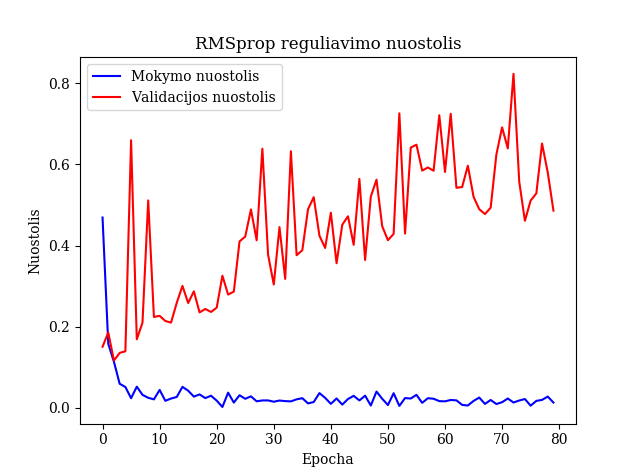
\includegraphics[width=\textwidth]{img/FT/RMSprop_loss.png}
    \caption{Modelio mokymosi ir validacijos nuostolis naudojant RMSprop}
  \end{minipage}
\end{figure}

Tad, tikslumo grafikas (9 pav.) parodo, kad mokymosi funkcija šokteli iki 100 procentų ir ten išsilaiko, kai validacijos funkcija stipriai svyruoja tarp 93 ir 95 procentų, bet per visas epochas neišsilygina.
O nuostolio grafikas (10 pav.) parodo, kad mokymosi funkcija nukrenta iki beveik 0 procentų ir ten išsilaiko. Tačiau validacijos funkcija labai stipriai svyruoja ir didėja. Pasiekdama aukščiausią nuostolį ties 82 procentais.

\subsubsection{Modelio modifikavimas}
Iš naujo apmokyti modeliai su 14 papildomų sluoksnių. Visi parametrai ir duomenų rinkinys liko tokie patys tik optimizavimo funkcija vėl buvo keičiama.

Tad, kaip ir prieš tai pirmoji modifikavimo funkcija yra SGD. Jos grafikai yra 11 ir 12 paveiksliukai.

\begin{figure}[!htbp]
  \centering
  \begin{minipage}[b]{0.49\textwidth}
    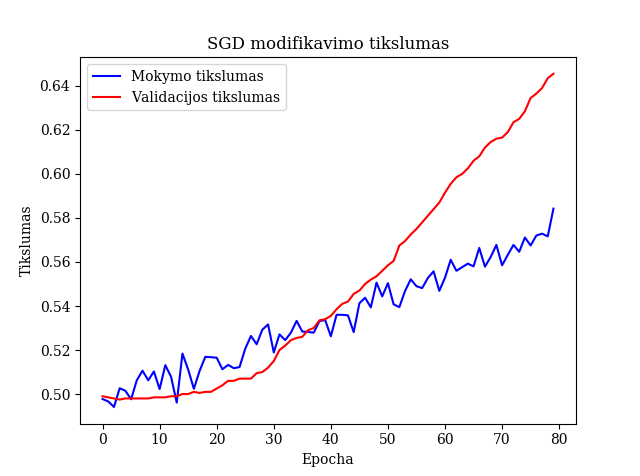
\includegraphics[width=\textwidth]{img/AL/SGD_acc.png}
    \caption{Gilesnio modelio mokymosi ir validacijos tikslumas naudojant SGD}
  \end{minipage}
  \begin{minipage}[b]{0.49\textwidth}
    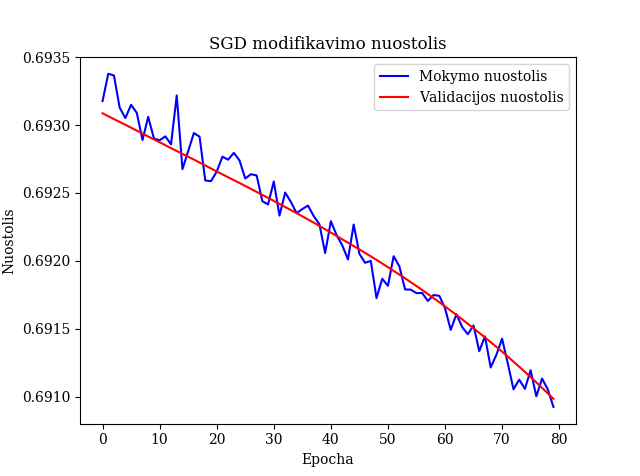
\includegraphics[width=\textwidth]{img/AL/SGD_loss.png}
    \caption{Gilesnio modelio mokymosi ir validacijos nuostolis naudojant SGD}
  \end{minipage}
\end{figure}

Tikslumo grafikas (11 pav.) matyti, kad mokymosi funkcija tolygiai svyruojančiai didėja, tačiau validacijos tikslumas ties 37 epocha pranoksta mokymosi bei pati validacijos funkcija tolygiai kyla ir neturi 
tokių svyravimų kaip mokymosi. Beje, palyginus su 3 paveiksliuko tikslumu, po papildomų sluoksnių pridėjimo nei validacijos nei mokymosi tikslumas nepasiekia tokio aukšto tikslumo, koks buvo mažesnio gylio modelyje.
Nuostolio grafike (12 pav.) parodyta, kad mokymosi ir validacijos funkcijos tolygiai mažėja, tačiau mokymosi svyruoja. Tačiau mažiausias nuostolis šiame grafike yra 69 procentai, kai 4 paveiksliuke, kur parodyta 
netokio gilaus modelio nuostoliai, mažiausi pasiekti nuostoliai yra 20 procentų.

Antra bandoma optimizavimo funkcija yra Adam. Jos grafikai yra 13 ir 14 paveiksliukai.

\begin{figure}[!htbp]
  \centering
  \begin{minipage}[b]{0.49\textwidth}
    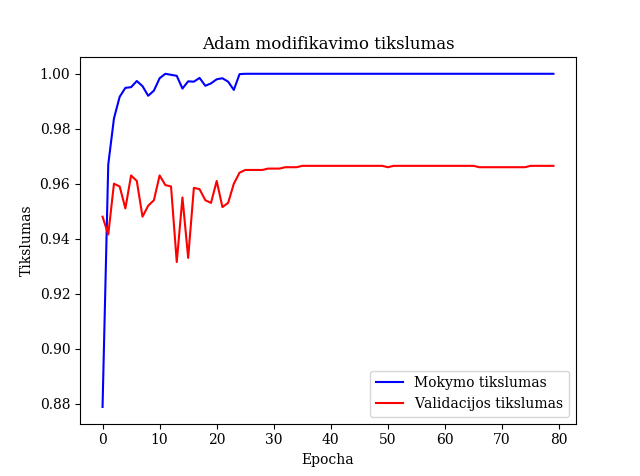
\includegraphics[width=\textwidth]{img/AL/Adam_acc.png}
    \caption{Gilesnio modelio mokymosi ir validacijos tikslumas naudojant Adam}
  \end{minipage}
  \begin{minipage}[b]{0.49\textwidth}
    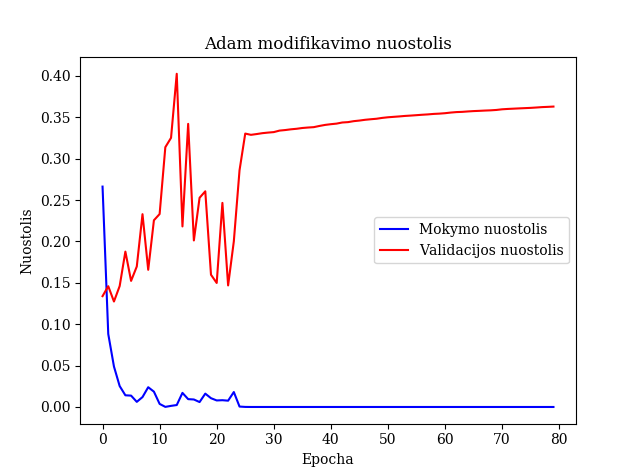
\includegraphics[width=\textwidth]{img/AL/Adam_loss.png}
    \caption{Gilesnio modelio mokymosi ir validacijos nuostolis naudojant Adam}
  \end{minipage}
\end{figure}

Taigi, tikslumo grafiką (13 pav.) palyginus su 5 paveiksliuku matyti, kad mokymosi tikslumo funkcija pakilo iki 100 procentų, panašiu greičiu. Beje, validacijos funkcija gilesniame modelyje pirmose 25 epochų ganėtinai 
stipriai svyravo, tačiau po to išsilygino ties 96 procentais. 
Tačiau nuostolio grafikas (14 pav.) labai skiriasi nuo 6 paveiksliuko, kur parodyta ne tokio gilaus modelio nuostolis. Mokymosi funkcija kaip ir mažesnio gylio modelio mažėja iki 0 procentų, tačiau validacijos nuostolis 
daug stipriau svyruoja pirmose 25 epochose, o po to išsilygina ir pradeda tolygiai didėti, pasiekdama didžiausia nuostolį ties 36 procentais.

Prieš paskutinė funkcija yra Adagrad. Šios funkcijos grafikai yra 15 ir 16 paveiksliukai.

\begin{figure}[!htbp]
  \centering
  \begin{minipage}[b]{0.49\textwidth}
    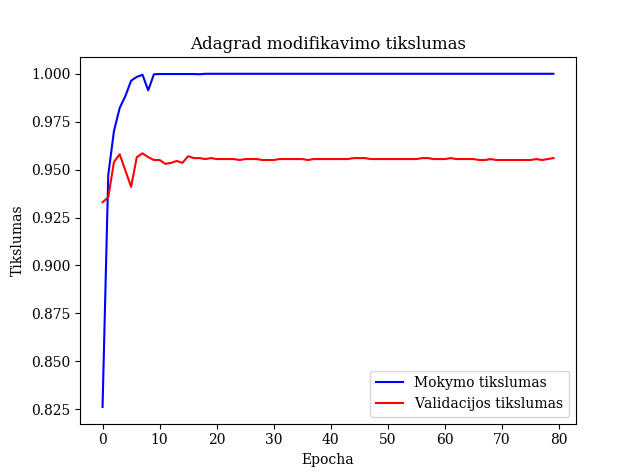
\includegraphics[width=\textwidth]{img/AL/Adagrad_acc.png}
    \caption{Gilesnio modelio mokymosi ir validacijos tikslumas naudojant Adagrad}
  \end{minipage}
  \begin{minipage}[b]{0.49\textwidth}
    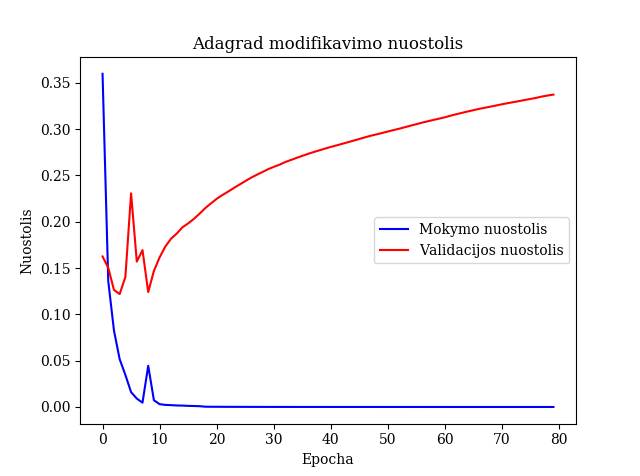
\includegraphics[width=\textwidth]{img/AL/Adagrad_loss.png}
    \caption{Gilesnio modelio mokymosi ir validacijos nuostolis naudojant Adagrad}
  \end{minipage}
\end{figure}

Tikslumo grafikas (15 pav.) yra labai panašus į mažesnio gylio tikslumo grafiką (7 pav.), kadangi mokymosi tikslumo funkcijos yra beveik vienodos, o validacija šiuo atveju yra šiek tiek mažesnio tikslumo gilesniame 
modelyje - susilygina ties 95 procentais.
Nuostolio grafikas (16 pav.) kaip ir 8 paveiksliuke, parodo, kad mokymosi nuostolis staigiai mažėja iki 0 procentų. O validacijos nuostolis pirmose 10 epochų stipriai svyruoja ir po to sparčiai auga ir pasiekia maksimalią nuostolio 
reikšmę ties 34 procentais, kai mažesnio gylio modelio yra apie 15 procentų.

Paskutinė optimizavimo funkcija yra RMSprop. Jos grafikai yra 17 ir 18 paveiksliukai.

\begin{figure}[!htbp]
  \centering
  \begin{minipage}[b]{0.49\textwidth}
    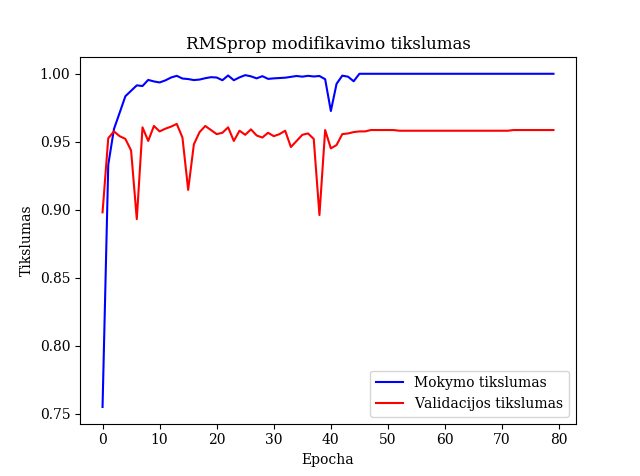
\includegraphics[width=\textwidth]{img/AL/RMSprop_acc.png}
    \caption{Gilesnio modelio mokymosi ir validacijos tikslumas naudojant RMSprop}
  \end{minipage}
  \begin{minipage}[b]{0.49\textwidth}
    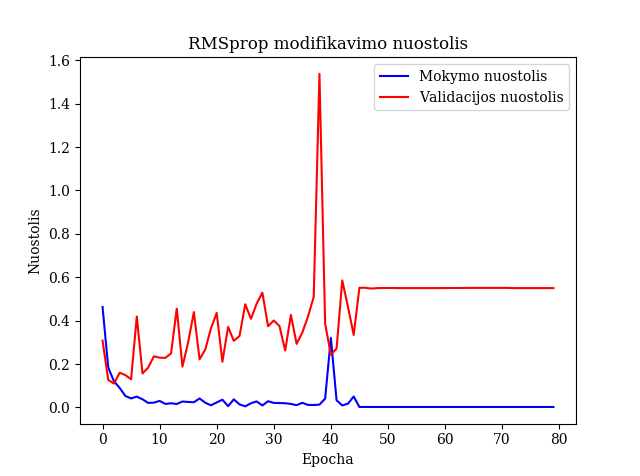
\includegraphics[width=\textwidth]{img/AL/RMSprop_loss.png}
    \caption{Gilesnio modelio mokymosi ir validacijos nuostolis naudojant RMSprop}
  \end{minipage}
\end{figure}

Tad, tikslumo grafike (17 pav.) matyti, kad mokymosi funkcija pakyla iki 100 procentų, o validacijos funkcija svyruoja iki 40 epochos, o po to išsilygina ties 95 procentais, kai toks pat rezultatą matomas ir 9 paveikslėlyje, kuriame parodyta mažiau gilaus modelio tikslumas.
O nuostolio grafikas (18 pav.) parodyta, kad mokymosi funkcija pasiekia 0 procentų. Tačiau validacijos funkcija svyruoja pirmas 45 epochas, o po to išsilygina ties 55 procentais.

\sectionnonum{Rezultatai ir išvados}
Darbo rezultatai:
\begin{itemize}
\item Pasirinktas tiriamas konvoliucinis neuroninis tinklas - VGG.
\item Sukurta programą, kuri reguliuotų ir modifikuotų pasirinktą konvoliucinį neuroninį tinklą.
\item Apmokytas reguliuotas ir modifikuotas modelis.
\item Mokymo metu buvo keičiamos optimizavimo funckijos - iš viso panaudotos SGD, Adam, Adagrad ir RMSprop funckijos.
\item Gauti modelio mokymo ir validacijos tikslumo ir nuostolio grafikai.
\end{itemize}

\hfill\break

Darbo išvados:
\begin{itemize}
\item Apmokius skirtingų gylių neuroninius tinklus, buvo nustatyta, kad gilesnis tinklas mokomojoje dalyje pasirodo labai gerai - tikslumas auga ir nuostolis mažėja iki 0 procentų, tačiau 
validacijos metu tikslumas pakyla iki tam tikros reikšmės ir pasidaro pastovus, o praradimas tolygiai auga. Galima daryti išvadą, kad gilesnis neuroninis tinklas su mažu kiekiu duomenų gali juos 
įsiminti, o ne išmokti atpažinti.
\item Mažo gylio modeliuose geriausia naudoti Adagrad optimizavimo funckiją, kadangi jos pasiektas validacijos tikslumas yra 96 procentai, nors ir Adam funkcija pasiekė tokį 
patį tikslumą. Tačiau Adam funkcijos validacijos nuostolis 80 epochoje siekė 25 procentus, kai Adagrad siekė tik 15 procentų ir augimo tendencija buvo daug mažensė.
\item Didesnio gylio modeliuose geriau naudoti Adam optimizavimo funkciją, kadangi validacijos tikslumas yra 96 procentai, o nuostolio funkcija pasiekia 35 procentus. O Adagrad 
funkcija pasiekia tikslumą 95 procentų ir nuostolį 35 procentų, tačiau turi labai didelę augimo tendenciją.
\end{itemize}

\printbibliography[heading=bibintoc] 

\end{document}
